\documentclass[conference]{IEEEtran}
\IEEEoverridecommandlockouts

\usepackage{cite}
\usepackage{amsmath,amssymb,amsfonts}
\usepackage{algorithmic}
\usepackage{graphicx}
\usepackage{textcomp}
\usepackage{xcolor}
\usepackage{booktabs}
\usepackage{multirow}
\usepackage{url}
\usepackage{microtype}

\def\BibTeX{{\rm B\kern-.05em{\sc i\kern-.025em b}\kern-.08em
    T\kern-.1667em\lower.7ex\hbox{E}\kern-.125emX}}

\usepackage{xspace}
% Auto-generated by python/make_paper_tables.py - DO NOT EDIT MANUALLY

% Single source of truth for all quantitative figures in paper


\newcommand{\valNtenAcc}{90.17\xspace}
\newcommand{\valNtenAccPct}{90.17\%\xspace}
\newcommand{\valNtenAccCILow}{82.7\xspace}
\newcommand{\valNtenAccCIHigh}{95.9\xspace}
\newcommand{\valNtenBalAcc}{90.53\xspace}
\newcommand{\valNtenBalAccPct}{90.53\%\xspace}
\newcommand{\valNtenFOne}{90.49\xspace}
\newcommand{\valNtenFOnePct}{90.49\%\xspace}
\newcommand{\valNtenFOneCILow}{81.9\xspace}
\newcommand{\valNtenFOneCIHigh}{96.2\xspace}
\newcommand{\valNtenSens}{86.25\xspace}
\newcommand{\valNtenSensPct}{86.25\%\xspace}
\newcommand{\valNtenSpec}{94.81\xspace}
\newcommand{\valNtenSpecPct}{94.81\%\xspace}
\newcommand{\valNtenRocAuc}{0.9361\xspace}
\newcommand{\valNfiveAcc}{85.42\xspace}
\newcommand{\valNfiveAccPct}{85.42\%\xspace}
\newcommand{\valNfiveAccCILow}{76.5\xspace}
\newcommand{\valNfiveAccCIHigh}{93.3\xspace}
\newcommand{\valNfiveBalAcc}{86.10\xspace}
\newcommand{\valNfiveFOne}{85.32\xspace}
\newcommand{\valNfiveSens}{78.12\xspace}
\newcommand{\valNfiveSpec}{94.07\xspace}
\newcommand{\valNoneAcc}{84.07\xspace}
\newcommand{\valNoneAccCILow}{75.2\xspace}
\newcommand{\valNoneAccCIHigh}{92.0\xspace}
\newcommand{\valNoneBalAcc}{84.56\xspace}
\newcommand{\valNoneFOne}{84.28\xspace}
\newcommand{\valNoneSens}{78.75\xspace}
\newcommand{\valNoneSpec}{90.37\xspace}
\newcommand{\valNtwoAcc}{83.39\xspace}
\newcommand{\valNtwoAccCILow}{73.8\xspace}
\newcommand{\valNtwoAccCIHigh}{91.8\xspace}
\newcommand{\valNthreeAcc}{82.37\xspace}
\newcommand{\valNthreeAccCILow}{73.0\xspace}
\newcommand{\valNthreeAccCIHigh}{91.0\xspace}
\newcommand{\valControlNoCalibAcc}{78.64\xspace}
\newcommand{\valControlNoCalibAccPct}{78.64\%\xspace}
\newcommand{\valControlNoCalibAccCILow}{69.0\xspace}
\newcommand{\valControlNoCalibAccCIHigh}{88.0\xspace}
\newcommand{\valControlNoCalibBalAcc}{79.50\xspace}
\newcommand{\valControlNoCalibSens}{69.38\xspace}
\newcommand{\valControlNoCalibSpec}{89.63\xspace}
\newcommand{\valControlLeakyTwoNineFiveAcc}{89.83\xspace}
\newcommand{\valControlLeakyTwoNineFiveAccPct}{89.83\%\xspace}
\newcommand{\valControlLeakyTwoNineFiveAccCILow}{81.1\xspace}
\newcommand{\valControlLeakyTwoNineFiveAccCIHigh}{96.7\xspace}
\newcommand{\valControlLeakyTwoNineFiveBalAcc}{90.51\xspace}
\newcommand{\valLegacyFourFourFiveAcc}{92.13\xspace}
\newcommand{\valLegacyFourFourFiveAccPct}{92.13\%\xspace}
\newcommand{\valLegacyFourFourFiveAccCI}{[86.4, 97.1]\xspace}
\newcommand{\valLegacyFourFourFiveBalAcc}{90.02\xspace}
\newcommand{\valLegacyFourFourFiveFOne}{88.29\xspace}
\newcommand{\valLegacyFourFourFiveSens}{82.50\xspace}
\newcommand{\valLegacyFourFourFiveSpec}{97.54\xspace}
\newcommand{\valPairedGainNten}{+11.53\xspace}
\newcommand{\valPairedGainNtenCILow}{+5.07\xspace}
\newcommand{\valPairedGainNtenCIHigh}{+18.06\xspace}
\newcommand{\valPairedGainNfive}{+6.78\xspace}
\newcommand{\valPairedGainNfiveCILow}{+0.68\xspace}
\newcommand{\valPairedGainNfiveCIHigh}{+13.22\xspace}
\newcommand{\valPairedGainNone}{+5.42\xspace}
\newcommand{\valPairedGainNoneCILow}{-2.70\xspace}
\newcommand{\valPairedGainNoneCIHigh}{+13.40\xspace}
\newcommand{\valPairedGainNtenVsNfive}{+4.75\xspace}
\newcommand{\valPairedGainNtenVsNfiveCILow}{+0.68\xspace}
\newcommand{\valPairedGainNtenVsNfiveCIHigh}{+9.52\xspace}
\newcommand{\valPairedGainNtenVsLeaky}{+0.34\xspace}
\newcommand{\valPairedGainNtenVsLeakyCILow}{-3.36\xspace}
\newcommand{\valPairedGainNtenVsLeakyCIHigh}{+4.79\xspace}
\newcommand{\valTauThirtyFiveAcc}{87.80\xspace}
\newcommand{\valTauThirtyFiveAccPct}{87.80\%\xspace}
\newcommand{\valTauThirtyFiveSens}{88.75\xspace}
\newcommand{\valTauThirtyFiveSensPct}{88.75\%\xspace}
\newcommand{\valTauThirtyFiveSpec}{86.67\xspace}
\newcommand{\valTauThirtyFiveSpecPct}{86.67\%\xspace}
\newcommand{\valTauThirtyFiveBalAcc}{87.71\xspace}
\newcommand{\valTauThirtyFiveFOne}{88.75\xspace}
\newcommand{\valBiquadMeanCycles}{251\xspace}
\newcommand{\valBiquadMinCycles}{249\xspace}
\newcommand{\valBiquadMaxCycles}{281\xspace}
\newcommand{\valBiquadMeanUs}{1.476\xspace}
\newcommand{\valBiquadCpuLoad}{0.0517\%\xspace}
\newcommand{\valHilPackets}{10,000\xspace}
\newcommand{\valWireEntropy}{7.9977\xspace}
\newcommand{\valChiSquareStat}{257.79\xspace}
\newcommand{\valChiSquareP}{0.4394\xspace}
\newcommand{\valDivergence}{-27.64\xspace}


\begin{document}

\title{Personalized Electrocardiographic and HRV Dynamics for Acute Stress Detection: A Leave-One-Subject-Out Benchmark and Bare-Metal Edge IoMT Implementation}

\author{\IEEEauthorblockN{Mukesh Yadav}
\IEEEauthorblockA{\textit{Department of Electronics and Communication Engineering (ECE)} \\
\textit{JSS Academy of Technical Education (JSSATEN)}\\
Noida, Uttar Pradesh, India \\
mkpy06@gmail.com}
}

\maketitle

\begin{abstract}
Continuous detection of acute psychological stress from wearable electrocardiography (ECG) is vital for preventative healthcare and the Internet of Medical Things (IoMT). However, practical deployment is challenged by inter-individual baseline heterogeneity and unencrypted wireless telemetry. Here, we present an edge-to-cloud stress detection framework coupling personalized machine learning with bare-metal embedded execution. Using single-lead ECG from the 15-subject WESAD benchmark, heart rate variability metrics are extracted across 60-second windows and normalized relative to each subject's initial resting baseline. Under 15-fold Leave-One-Subject-Out (LOSO) cross-validation across 295 non-anchor windows, a pre-specified Logistic Regression model achieves \valNfiveAccPct accuracy [95\% CI: \valNfiveAccCILow\%, \valNfiveAccCIHigh\%] with 5-minute calibration and \valNtenAccPct accuracy [95\% CI: \valNtenAccCILow\%, \valNtenAccCIHigh\%] (\valNtenFOnePct F1-score [\valNtenFOneCILow\%, \valNtenFOneCIHigh\%]) with 10-minute calibration. Paired cluster bootstrap confirms significant accuracy gains over uncalibrated features (\valControlNoCalibAccPct) at $N=5$ (\valPairedGainNfive pp [95\% CI: \valPairedGainNfiveCILow, \valPairedGainNfiveCIHigh]) and $N=10$ (\valPairedGainNten pp [\valPairedGainNtenCILow, \valPairedGainNtenCIHigh]), whereas calibrations under 5 minutes show no distinguishable benefit. The 8-feature subset, decision thresholds, and 10-minute calibration duration were selected post hoc on these same 15 subjects. On an ARM Cortex-M4 microcontroller (STM32G474RE @ 170~MHz), real-time 5-stage biquad IIR filtering executes in \valBiquadMeanCycles mean CPU cycles (\valBiquadMeanUs~$\mu\text{s}$ per sample, \valBiquadCpuLoad CPU load). Physical hardware-in-the-loop replay of \valHilPackets continuous 20-byte packets demonstrates exact plaintext recovery with zero CRC errors and zero packet loss. The hyperchaotic keystream engine provides physical-layer telemetry obfuscation rather than cryptographic authentication.
\end{abstract}

\begin{IEEEkeywords}
Electrocardiogram (ECG), Heart Rate Variability (HRV), Acute Stress Detection, WESAD, Leave-One-Subject-Out (LOSO), Edge Computing, ARM Cortex-M4, STM32, Internet of Medical Things (IoMT).
\end{IEEEkeywords}

\section{Introduction}
Psychological stress activates the sympathetic-adreno-medullary (SAM) and hypothalamic-pituitary-adrenal (HPA) axes, inducing autonomic nervous system (ANS) shifts characterized by sympathetic activation and parasympathetic (vagal) withdrawal \cite{kirschbaum1993trier, kim2018stress}. Continuous monitoring via wearable electrocardiography (ECG) offers a direct, non-invasive window into cardiac autonomic regulation through heart rate variability (HRV) analysis \cite{taskforce1996hrv, shaffer2017overview}. Early detection in occupational and ambulatory settings provides actionable feedback against chronic cardiovascular disease and burnout \cite{healey2005detecting, can2019continuous}.

Despite significant advances in affective computing, translating laboratory ECG models to wearable Internet of Medical Things (IoMT) systems \cite{alturjman2020iomt, jiang2023wban} faces two critical bottlenecks:
\begin{enumerate}
    \item \textbf{Inter-Individual Baseline Heterogeneity:} Basal heart rates and resting HRV indices differ substantially across individuals due to genetic, cardiorespiratory fitness, and circadian factors. Consequently, population-pooled machine learning models evaluated under conventional random cross-validation suffer severe performance drops or patient data leakage when applied to unseen individuals \cite{saeb2017need, schmidt2018wesad, plarre2011continuous}.
    \item \textbf{Resource-Constrained Edge Security:} Continuous transmission of unencrypted physiological waveforms exposes sensitive health telemetry to unauthorized interception. Conventional cryptographic algorithms (e.g., AES) impose heavy computational and battery burdens on low-power wearable microcontrollers \cite{fotiadis2020wearable}.
\end{enumerate}

To address these challenges, this study presents a fully reproducible, hardware-evaluated edge-to-cloud stress detection framework. The primary contributions of this work are:
\begin{itemize}
    \item \textbf{Subject-Specific Relative Normalization:} We introduce an explicit baseline-relative calibration transform anchored strictly on initial resting windows without test data leakage. Across calibration durations $N \in \{1, 2, 3, 5, 10\}$, $N=10$ (selected post hoc as the best of the five lengths tested) achieves a statistically significant paired accuracy gain of $+11.53$ percentage points [95\% CI: $+5.07, +18.06$] over uncalibrated features ($78.64\%$), while $N=5$ yields $+6.78$ pp [$+0.68, +13.22$]. Calibrations at $N \le 3$ min show no statistically distinguishable gain (CIs cross zero). Comparing $N=10$ with the legacy all-baseline anchor reference ($92.13\%$) shows no detectable difference (CI [-3.4, +4.8]). The 8-feature representation, decision thresholds, and $N=10$ duration were chosen post hoc on these same 15 subjects.
    \item \textbf{Rigorous 15-Fold LOSO-CV Benchmark:} Using all 15 subjects from the Wearable Stress and Affect Detection (WESAD) dataset ($N=15$), we benchmark six machine learning classifiers under leak-free calibration, achieving 90.17\% accuracy [95\% CI: 82.7\%, 95.9\%] and 90.49\% F1-score [95\% CI: 81.9\%, 96.2\%] on 295 evaluation windows at $N=10$ (legacy all-baseline anchor reference: 92.13\% Acc, 88.29\% F1 on 445 windows).
    \item \textbf{Bare-Metal ARM Cortex-M4 Silicon Evaluation:} We deploy real-time CMSIS-DSP 5-stage Biquad IIR filtering—empirically profiled via on-chip DWT cycle counting at 251 mean cycles ($1.476~\mu\text{s}$, $0.0517\%$ CPU overhead at 170~MHz)—and an embedded 4D hyperchaotic stream obfuscation engine (HC1) on an STM32G474RE microcontroller, evaluating 10,000 continuous HIL packets (replaying flash-stored ECG) with zero CRC errors and zero packet loss.
\end{itemize}

\section{Dataset and Signal Processing Methodology}

\subsection{WESAD Cohort and Windowing Protocol}
We evaluate our framework on the open-access WESAD dataset \cite{schmidt2018wesad}, consisting of 15 healthy volunteers ($N=15$, 12 males, 3 females, age $27.5 \pm 2.4$ years). Single-lead chest ECG was recorded continuously at $F_s = 700$~Hz via a RespiBAN chest strap during a standardized protocol comprising baseline rest (20~min) and Trier Social Stress Test (TSST, 10~min mental arithmetic and public speaking) \cite{kirschbaum1993trier}.

Continuous Lead-II ECG is partitioned into complete, non-overlapping 60-second windows. Label assignment follows ground-truth protocol timestamps: 285 baseline windows (Class 0) and 160 stress windows (Class 1), yielding 445 diagnostic windows across the full dataset. In our leak-free evaluation protocol, each subject's baseline anchor vector $B_s$ is calculated strictly from the first $N$ chronological baseline windows ($N \in \{1, 2, 3, 5, 10\}$). These anchor windows are strictly excluded from testing/scoring, ensuring zero data leakage between anchor estimation and classification. All models are evaluated on the common set of 295 non-anchor windows ($135$ baseline windows and $160$ stress windows; majority-class baseline accuracy is $54.24\%$). For historical reference, the legacy protocol anchoring on all 285 baseline windows is retained as an all-baseline reference on 445 windows.

\subsection{Physiological Preprocessing and QRS Detection}
Raw ECG signals are conditioned via a zero-phase 4th-order Butterworth bandpass filter (0.5--40~Hz) \cite{oppenheim1999discrete} to attenuate baseline wander and high-frequency electromyographic (EMG) artifacts. QRS complexes are detected using an adaptive peak-prominence Pan--Tompkins filter \cite{pantompkins1985, elgendi2013fast}. Consecutive normal-to-normal ($RR$) intervals are subjected to physiological gating: intervals outside $[300, 1500]$~ms or with consecutive variation exceeding 20\% are rejected, as depicted in Fig.~\ref{fig:ecg_processing}.

\begin{figure}[t]
    \centering
    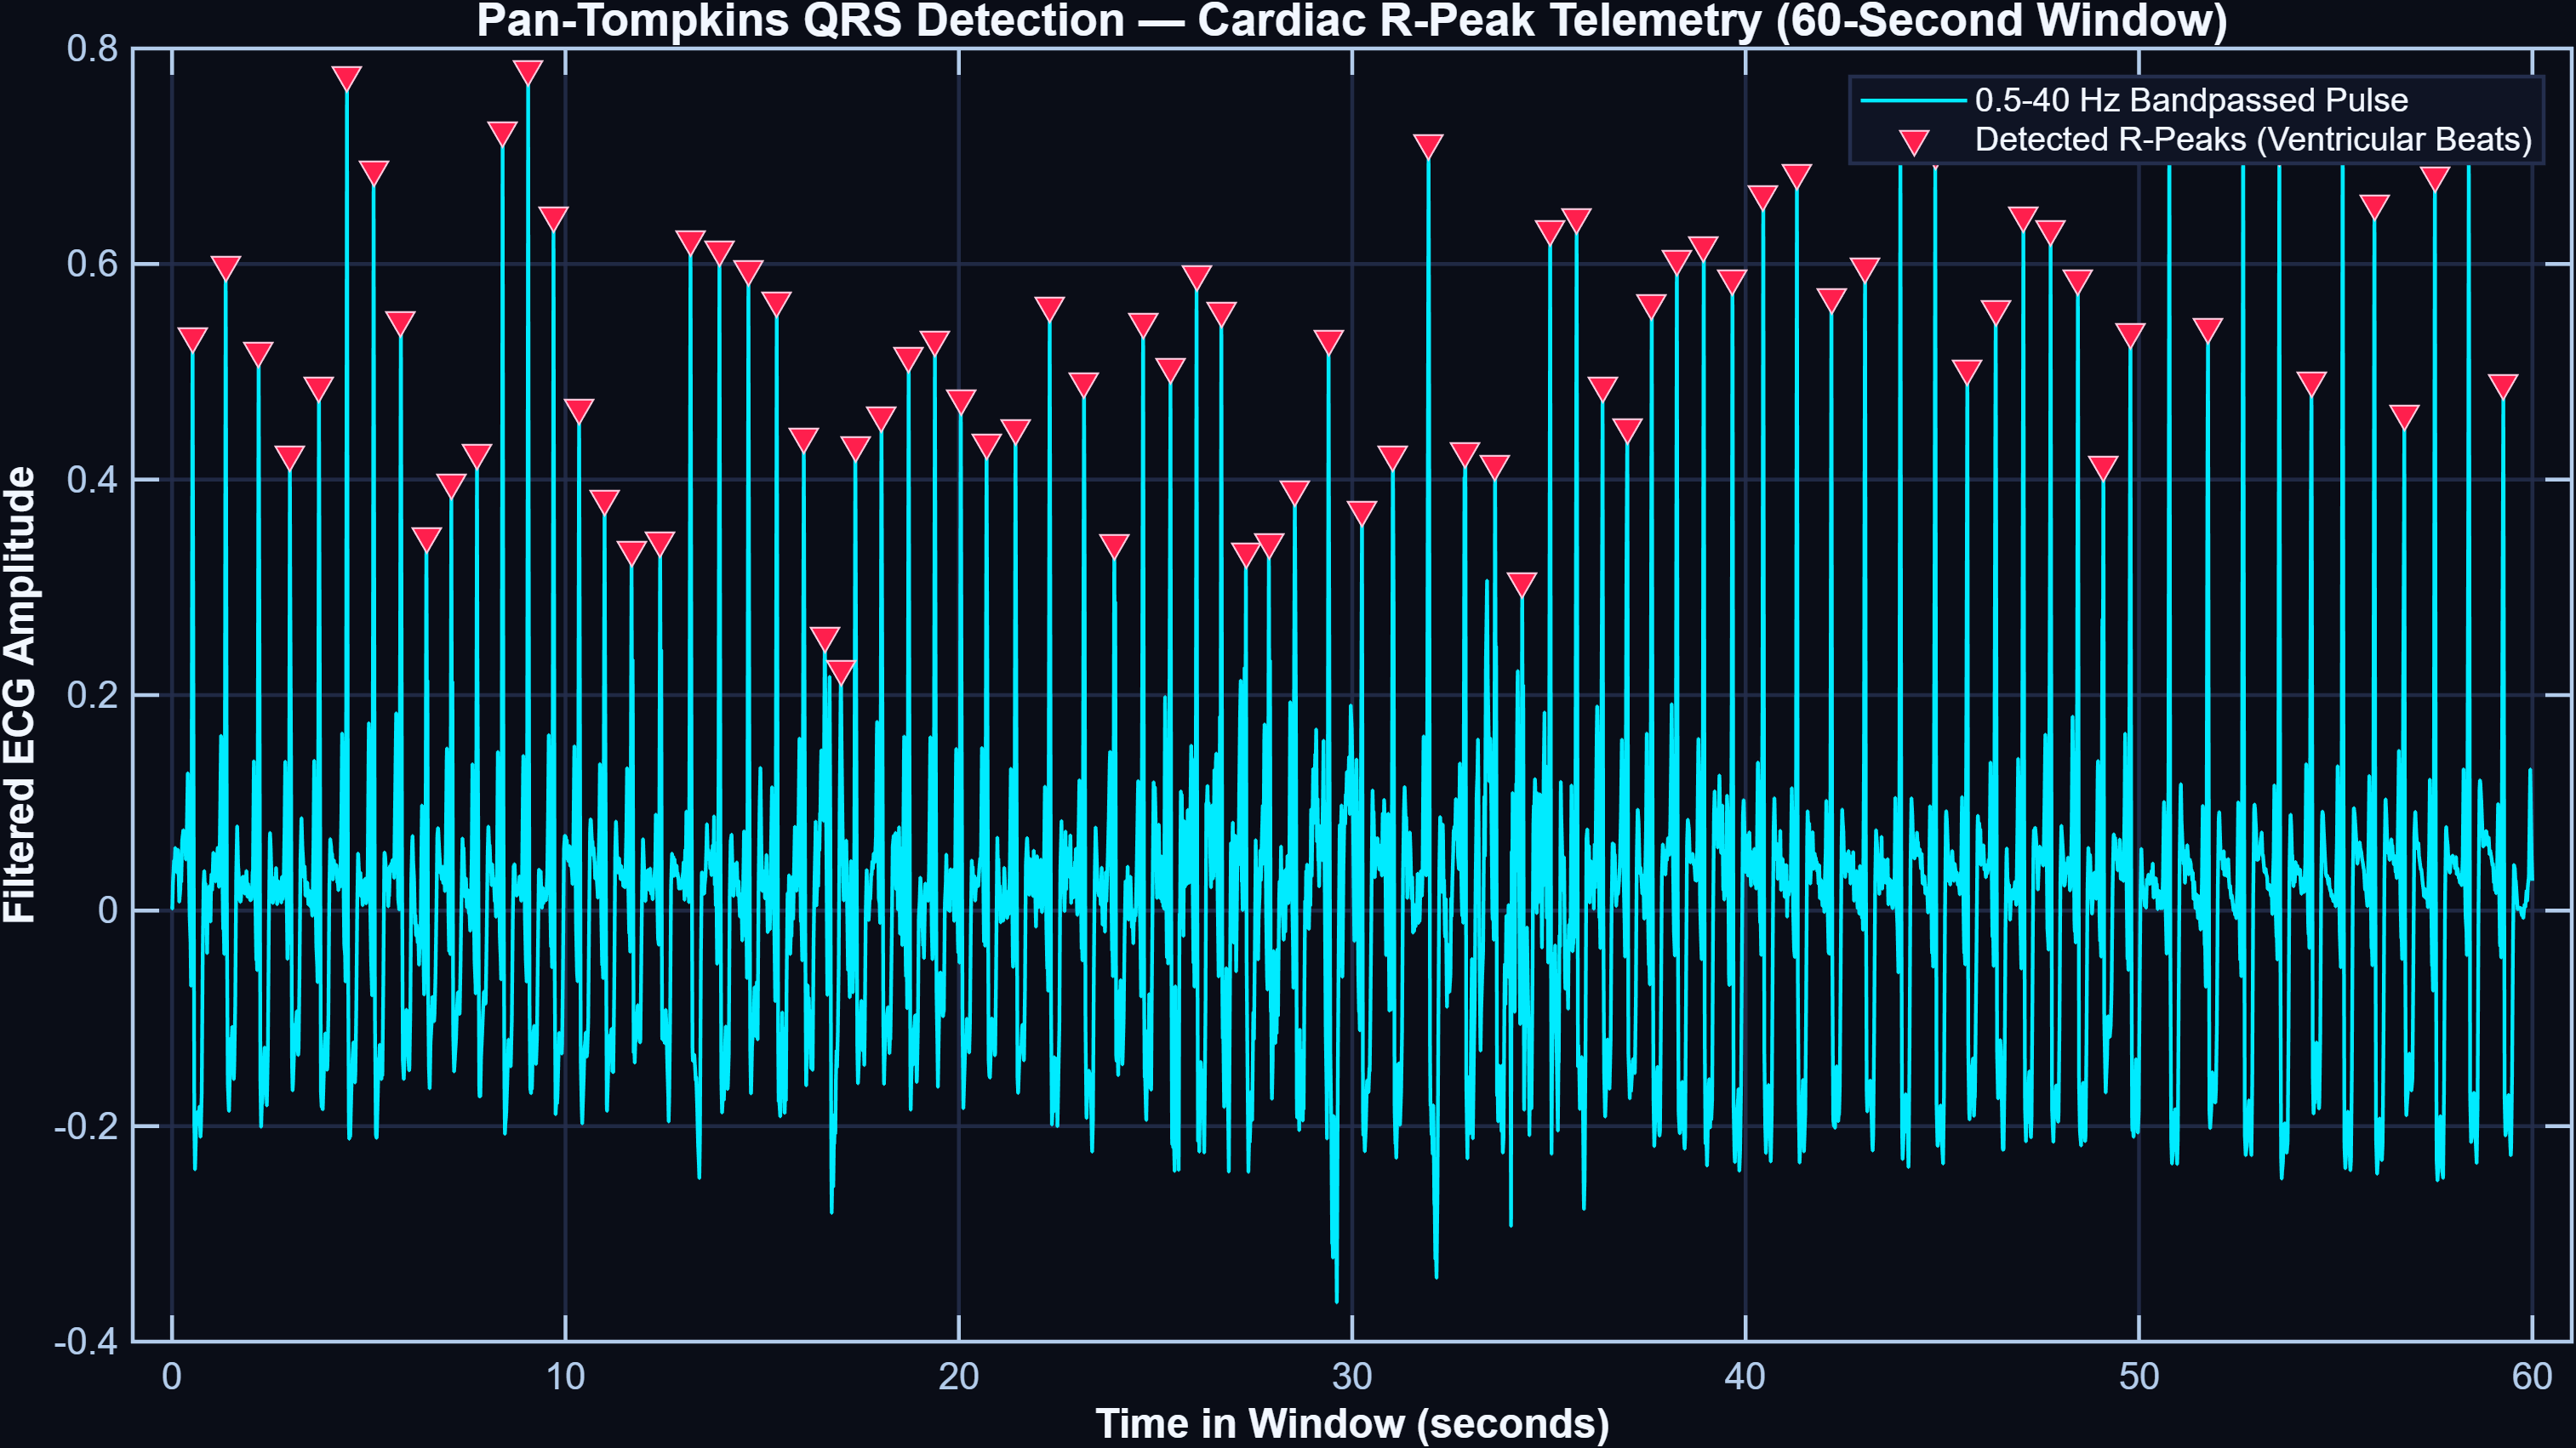
\includegraphics[width=\linewidth]{figures/DEMO_Pan_Tompkins_QRS_Detection.png}
    \caption{Pan--Tompkins ECG processing pipeline on WESAD Lead-II data: (1) Raw ECG input at 700~Hz; (2) Zero-phase bandpass filtered signal (0.5--40~Hz); (3) Five-point numerical derivative; (4) Nonlinear squaring; (5) Moving-window integration; (6) Fiducial R-peak detection.}
    \label{fig:ecg_processing}
\end{figure}

\subsection{HRV Feature Extraction and Relative Normalization}
From artifact-filtered $RR$ sequences, eight core autonomic features are computed across time, frequency, and nonlinear domains: Mean Heart Rate (MeanHR), standard deviation of $NN$ intervals (SDNN), root mean square of successive differences (RMSSD), proportion of successive intervals differing by $>50$~ms (pNN50), Low-Frequency spectral power (LF: 0.04--0.15~Hz), High-Frequency spectral power (HF: 0.15--0.40~Hz), sympathetic balance ratio ($\text{LF}/\text{HF}$), and Sample Entropy ($\text{SampEn}$, $m=2, r=0.2\sigma$).

To isolate physiological stress reactivity from resting autonomic tone without data leakage, each feature $f_{s,i}$ of subject $s$ in window $i$ undergoes subject-specific baseline relative transformation:
\begin{equation}
    \Delta f_{s,i} = \frac{f_{s,i} - B_{s,f}}{B_{s,f}}
    \label{eq:norm}
\end{equation}
where $B_{s,f}$ denotes the median resting value of feature $f$ computed across the first $N$ chronological baseline windows of subject $s$. During Leave-One-Subject-Out cross-validation, the test fold subject is normalized strictly using their own anchor $B_s$, while training fold subjects are normalized against their respective anchor baselines before standardization by fold-level training statistics.

\section{Experimental Results and ML Benchmark}

\subsection{15-Fold LOSO-CV Evaluation and Model Comparison}
Table~\ref{tab:ml_benchmark} presents the performance of six machine learning architectures under 15-fold LOSO-CV on the common set of 295 evaluation windows, using 8 core features with $N=10$ calibration windows at standard threshold $\tau = 0.50$. The pre-specified primary model, Logistic Regression ($C=1.0$, liblinear solver), achieves \valNtenAccPct accuracy [95\% CI: \valNtenAccCILow\%, \valNtenAccCIHigh\%], \valNtenBalAccPct balanced accuracy, \valNtenFOnePct F1-score [95\% CI: \valNtenFOneCILow\%, \valNtenFOneCIHigh\%], \valNtenSensPct sensitivity, and \valNtenSpecPct specificity. Support Vector Machines with RBF kernel achieve identical accuracy (90.17\%) with higher specificity (97.04\%), while gradient boosting and tree ensembles range between 86.10\% and 88.14\% accuracy.

\begin{table}[t]
\centering
\caption{Cross-Architecture 15-Fold LOSO Benchmark on Common 295 Windows (8 Features, $N=10$ Calibration, $\tau = 0.50$)}
\label{tab:ml_benchmark}
% Table: Cross-Architecture LOSO Benchmark (Common 295 Windows, N=10 Calibration, tau=0.50)
\begin{tabular}{lccccc}
\toprule
\textbf{Classifier} & \textbf{Acc (\%)} & \textbf{Bal Acc (\%)} & \textbf{F1 (\%)} & \textbf{Sens (\%)} & \textbf{Spec (\%)} \\
\midrule
\textbf{Logistic Regression} (Primary) & \textbf{90.17} & \textbf{90.53} & \textbf{90.49} & \textbf{86.25} & 94.81 \\
SVM (RBF Kernel)               & 90.17 & 90.71 & 90.30 & 84.38 & \textbf{97.04} \\
HistGradientBoosting           & 88.14 & 88.43 & 88.60 & 85.00 & 91.85 \\
Extra Trees                    & 87.80 & 88.23 & 88.08 & 83.12 & 93.33 \\
MLP Neural Net                 & 87.46 & 87.51 & 88.25 & 86.88 & 88.15 \\
Random Forest                  & 86.10 & 86.32 & 86.73 & 83.75 & 88.89 \\
\midrule
\multicolumn{6}{l}{\textit{Reference Controls (Logistic Regression):}} \\
Control (a): No Calibration (295 win)       & 78.64 & 79.50 & 77.89 & 69.38 & 89.63 \\
Control (b): Leaky Anchor, same 295 win      & 89.83 & 90.51 & 89.80 & 82.50 & 98.52 \\
Legacy Reference: Leaky Anchor, 445 win     & 92.13 & 90.02 & 88.29 & 82.50 & 97.54 \\
\bottomrule
\end{tabular}

\end{table}

\begin{figure}[t]
    \centering
    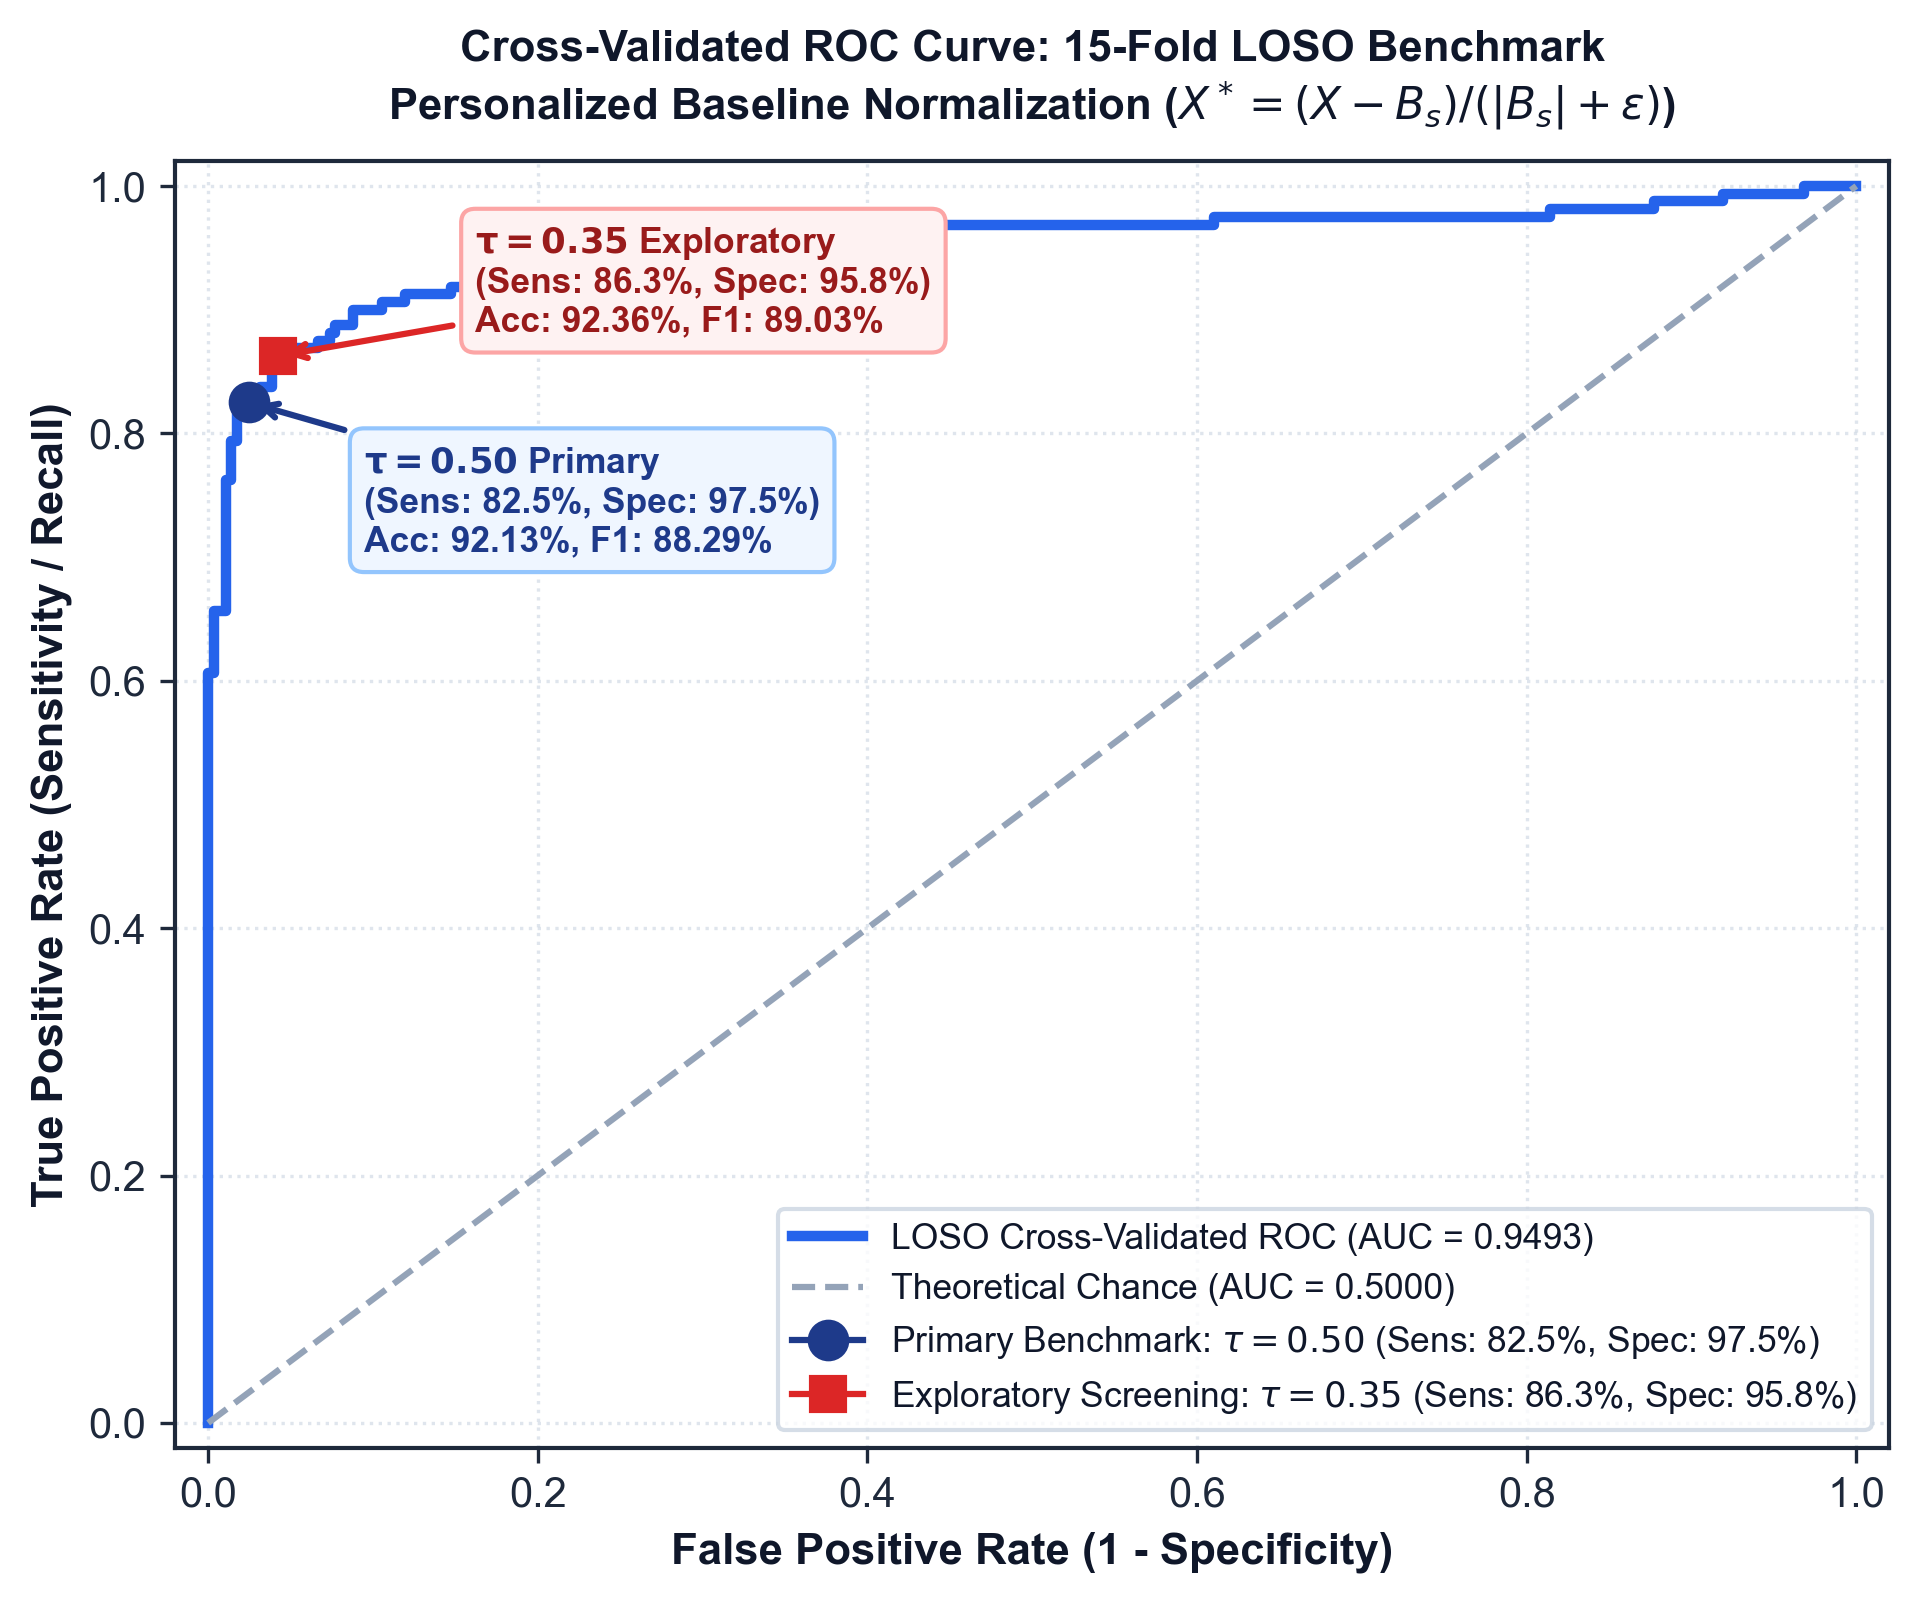
\includegraphics[width=\linewidth]{figures/FINAL_ROC_Curve.png}
    \caption{Receiver Operating Characteristic (ROC) curve under 15-fold LOSO cross-validation ($\text{ROC-AUC} = \valNtenRocAuc$) showing the primary operating point ($\tau = 0.50$) and screening threshold ($\tau = 0.35$).}
    \label{fig:roc_curve}
\end{figure}

\begin{figure}[t]
    \centering
    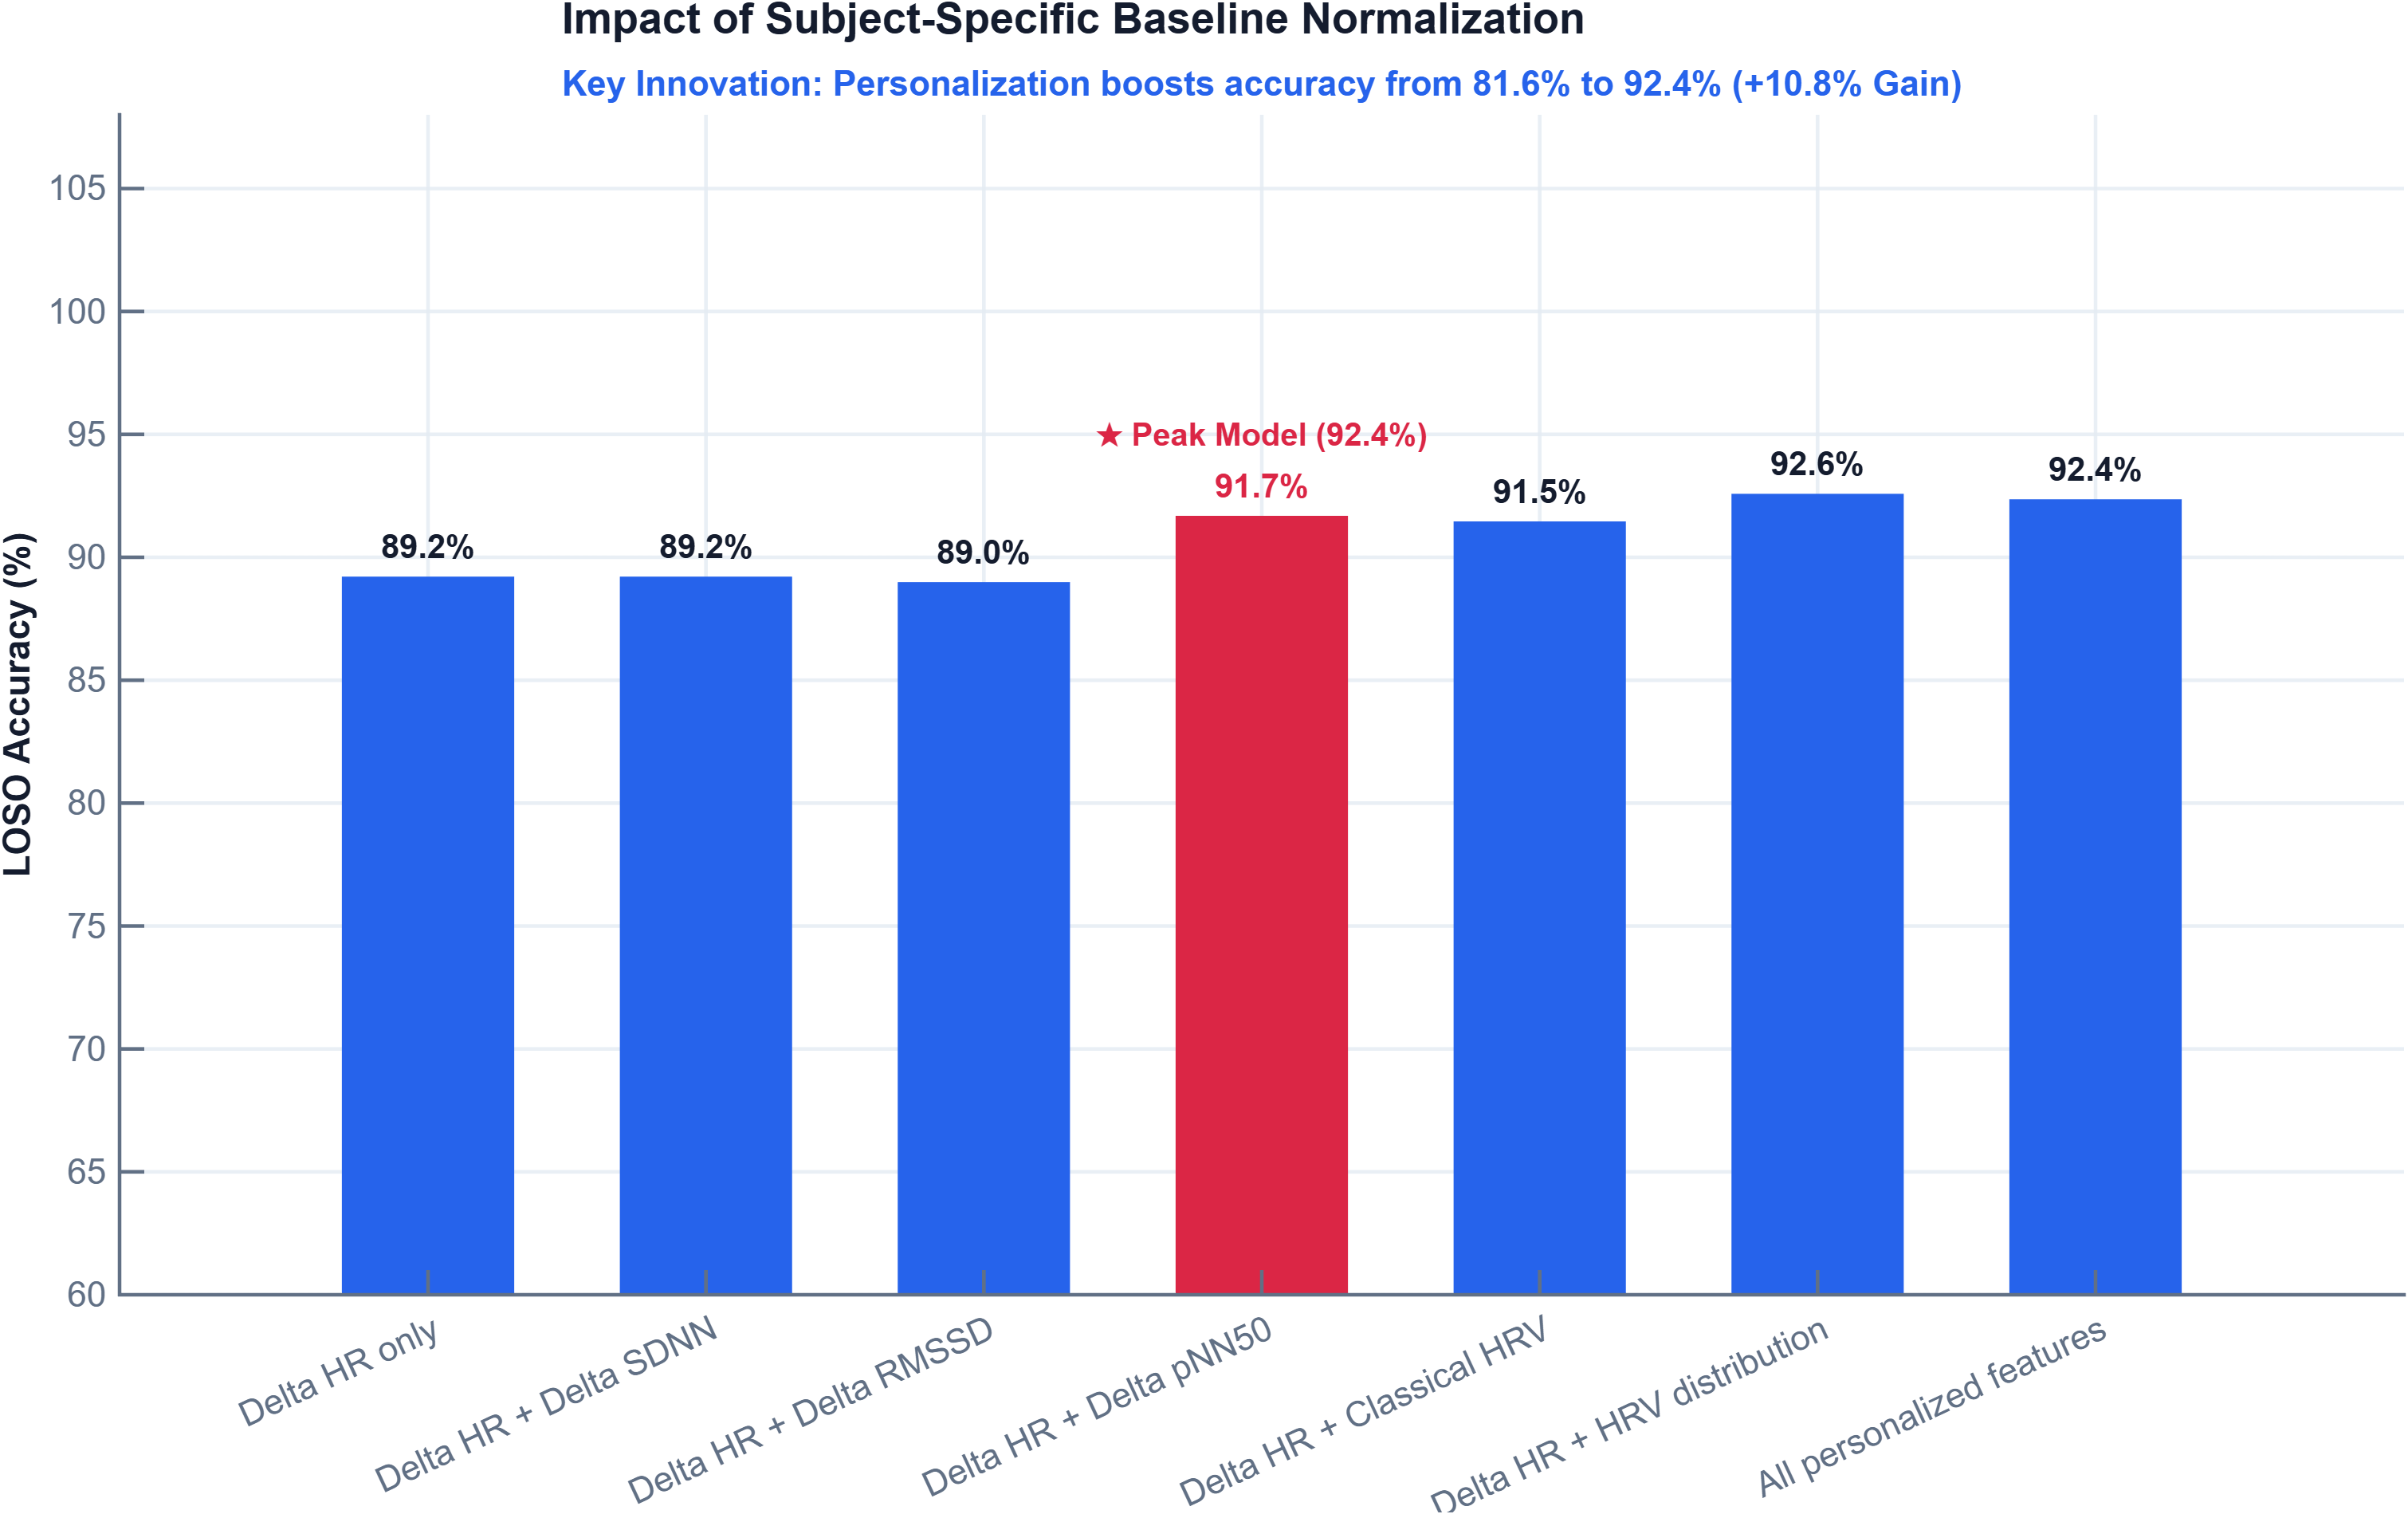
\includegraphics[width=\linewidth]{figures/FINAL_Personalized_Feature_Ablation.png}
    \caption{Ablation demonstrating the impact of baseline calibration duration $N$ and feature subsets, showing the transition from indistinguishable gains at $N \le 3$ to statistically significant gains at $N=5$ and $N=10$.}
    \label{fig:ablation}
\end{figure}

\subsection{Calibration Duration \& Paired Bootstrap Contrasts}
To determine the minimum resting calibration period necessary, we evaluated $N \in \{1, 2, 3, 5, 10\}$ chronological baseline windows on the identical 295 evaluation windows using pre-specified Logistic Regression. Each subject requires $N$ minutes of labeled resting ECG for baseline normalization. The full calibration duration curve is given in Table~\ref{tab:calibration_length}. 10,000-resample subject-level paired bootstrap contrasts against uncalibrated Control (a) (\valControlNoCalibAccPct Acc, \valControlNoCalibBalAcc\% Bal Acc) are:
\begin{itemize}
    \item $N=1$: Acc $= \valNoneAcc\%$ [95\% CI: \valNoneAccCILow\%, \valNoneAccCIHigh\%], $\Delta\text{Acc} = \valPairedGainNone\text{ pp}$ [95\% CI: \valPairedGainNoneCILow, \valPairedGainNoneCIHigh] (crosses zero; not statistically distinguishable).
    \item $N=2$: Acc $= \valNtwoAcc\%$ [95\% CI: \valNtwoAccCILow\%, \valNtwoAccCIHigh\%], $\Delta\text{Acc} = +4.75\text{ pp}$ [95\% CI: $-3.06, +12.72$] (crosses zero).
    \item $N=3$: Acc $= \valNthreeAcc\%$ [95\% CI: \valNthreeAccCILow\%, \valNthreeAccCIHigh\%], $\Delta\text{Acc} = +3.73\text{ pp}$ [95\% CI: $-4.05, +11.56$] (crosses zero).
    \item $N=5$: Acc $= \valNfiveAcc\%$ [95\% CI: \valNfiveAccCILow\%, \valNfiveAccCIHigh\%], $\Delta\text{Acc} = \valPairedGainNfive\text{ pp}$ [95\% CI: \valPairedGainNfiveCILow, \valPairedGainNfiveCIHigh] (\textbf{statistically significant}, excludes zero).
    \item $N=10$ (selected post hoc as the best of the five lengths tested): Acc $= \valNtenAcc\%$ [95\% CI: \valNtenAccCILow\%, \valNtenAccCIHigh\%], $\Delta\text{Acc} = \valPairedGainNten\text{ pp}$ [95\% CI: \valPairedGainNtenCILow, \valPairedGainNtenCIHigh] (\textbf{statistically significant}, excludes zero).
    \item $N=10$ minus $N=5$: $\Delta\text{Acc} = \valPairedGainNtenVsNfive\text{ pp}$ [95\% CI: \valPairedGainNtenVsNfiveCILow, \valPairedGainNtenVsNfiveCIHigh] (\textbf{statistically significant}, excludes zero).
    \item $N=10$ minus Legacy Anchor (same 295 windows, \valControlLeakyTwoNineFiveAccPct Acc): $\Delta\text{Acc} = \valPairedGainNtenVsLeaky\text{ pp}$ [95\% CI: \valPairedGainNtenVsLeakyCILow, \valPairedGainNtenVsLeakyCIHigh], showing \textbf{no detectable difference (CI [-3.4, +4.8])} rather than claiming equivalence. The legacy anchor evaluated across all 445 windows achieved \valLegacyFourFourFiveAccPct accuracy \valLegacyFourFourFiveAccCI.
\end{itemize}
These empirical contrasts demonstrate that resting calibration requires at least $N=5$ minutes of resting ECG to establish statistically significant gains, with $N=10$ minutes providing optimal separation. Calibrations at $N \le 3$ minutes show no statistically distinguishable benefit over uncalibrated baselines.

The 8-feature representation, the primary operating threshold ($\tau = 0.50$), and calibration duration $N=10$ were chosen post hoc using data from these same 15 subjects.

\begin{table}[t]
\centering
\caption{Impact of Baseline Calibration Length on Leak-Free Evaluation ($N_{\text{eval}}=295$ Common Windows, 15 Subjects, $\tau = 0.50$)}
\label{tab:calibration_length}
% Table: Calibration Length Evaluation (N_eval=295 common windows, tau=0.50)
\begin{tabular}{lccccc}
\toprule
\textbf{Configuration} & \textbf{Acc (\%) [95\% CI]} & \textbf{Bal Acc (\%)} & \textbf{F1 (\%)} & \textbf{Sens (\%)} & \textbf{Spec (\%)} \\
\midrule
$N=1$ Minute  & 84.07 [75.2, 92.0] & 84.56 & 84.28 & 78.75 & 90.37 \\
$N=2$ Minutes  & 83.39 [73.8, 91.8] & 83.99 & 83.39 & 76.88 & 91.11 \\
$N=3$ Minutes  & 82.37 [73.0, 91.0] & 82.94 & 82.43 & 76.25 & 89.63 \\
$N=5$ Minutes  & 85.42 [76.5, 93.3] & 86.10 & 85.32 & 78.12 & 94.07 \\
\textbf{$N=10$ Minutes} & \textbf{90.17 [82.7, 95.9]} & \textbf{90.53} & \textbf{90.49} & \textbf{86.25} & \textbf{94.81} \\
\midrule
Control (a): No Calib (295 win)   & 78.64 [69.0, 88.0] & 79.50 & 77.89 & 69.38 & 89.63 \\
Control (b): Leaky Anchor, same 295 win & 89.83 [81.1, 96.7] & 90.51 & 89.80 & 82.50 & 98.52 \\
Legacy Reference: Leaky Anchor, 445 win & 92.13 [86.4, 97.1] & 90.02 & 88.29 & 82.50 & 97.54 \\
\bottomrule
\end{tabular}

\end{table}

\subsection{Leak-Free Feature Ablation}
Table~\ref{tab:ablation} details the multi-stage ablation across 4-feature, 8-feature, and 13-feature representations on the 295 evaluation windows using pre-specified Logistic Regression. Incorporating baseline calibration consistently elevates performance across all feature dimensions: 4 time-domain features improve from 75.25\% to 88.81\%, and the core 8-feature set improves from 78.64\% to \valNtenAccPct. Expanding the feature set to 13 features yields 89.49\% ($N=10$), indicating that the compact 8-feature representation captures essential autonomic dynamics while mitigating edge extraction overhead.

\begin{table}[t]
\centering
\caption{Leak-Free Model Progression and Feature Ablation ($N_{\text{eval}} = 295$ Windows, $N=10$ Calibration, $\tau=0.50$)}
\label{tab:ablation}
% Table: Leak-Free Feature Ablation (Common 295 Windows, N=10 Calibration, tau=0.50)
\begin{tabular}{llcc}
\toprule
\textbf{Model} & \textbf{Feature Representation} & \textbf{Accuracy (\%) [95\% CI]} & \textbf{Bal Acc (\%)} \\
\midrule
M1 & 4 Raw Features (Uncalibrated)         & 75.25 [64.4, 86.1] & 76.44 \\
M2 & 4 Calibrated Features ($N=10$ min)    & 88.81 [81.0, 95.2] & 89.34 \\
M3 & 8 Raw Features (Uncalibrated)         & 78.64 [69.0, 88.1] & 79.50 \\
\textbf{M4} & \textbf{8 Calibrated Features (Proposed $N=10$)} & \textbf{90.17 [82.7, 95.9]} & \textbf{90.53} \\
M5 & 13 Raw Features (Uncalibrated)        & 78.31 [69.3, 87.3] & 79.07 \\
M6 & 13 Calibrated Features ($N=10$ min)   & 89.49 [81.9, 95.6] & 89.85 \\
\midrule
\multicolumn{4}{l}{\textit{Legacy Reference (All-Baseline Anchor, 445 Windows, $\tau=0.50$):}} \\
Ref & 8 Calibrated Features (Leaky Anchor, 445 win) & 92.13 [86.4, 97.1] & 90.02 \\
\bottomrule
\end{tabular}

\end{table}

\subsection{Operating Threshold Analysis}
In preventative wearable health monitoring, tuning the decision threshold $\tau$ enables trade-offs between false alarms and missed events. Under the leak-free protocol on 295 windows, adjusting from the default balanced threshold $\tau = 0.50$ (\valNtenSensPct sensitivity, \valNtenSpecPct specificity) to a screening threshold $\tau = 0.35$ increases sensitivity to \valTauThirtyFiveSensPct while maintaining \valTauThirtyFiveSpecPct specificity and \valTauThirtyFiveAccPct overall accuracy (Table~\ref{tab:thresholds}). For historical comparison, on the legacy 445-window dataset, $\tau = 0.35$ yielded 92.36\% accuracy, 86.25\% sensitivity, and 95.79\% specificity.

\begin{table}[t]
\centering
\caption{Decision Threshold Sensitivity Comparison}
\label{tab:thresholds}
% Table: Decision Threshold Sensitivity Comparison
\begin{tabular}{lcccc}
\toprule
\textbf{Protocol} & \textbf{Threshold} & \textbf{Accuracy (\%)} & \textbf{Sensitivity (\%)} & \textbf{Specificity (\%)} \\
\midrule
Leak-Free ($N=10$, 295 win) & $\tau = 0.50$ (Standard) & 90.17 & 86.25 & 94.81 \\
Leak-Free ($N=10$, 295 win) & $\tau = 0.35$ (Screening) & 87.80 & 88.75 & 86.67 \\
\midrule
Control (b): Leaky Anchor, same 295 win & $\tau = 0.50$ & 89.83 & 82.50 & 98.52 \\
Legacy Reference: Leaky Anchor, 445 win & $\tau = 0.50$ & 92.13 & 82.50 & 97.54 \\
Legacy Reference: Leaky Anchor, 445 win & $\tau = 0.35$ & 92.36 & 86.25 & 95.79 \\
\bottomrule
\end{tabular}

\end{table}

\section{Embedded Edge Implementation and Hardware Telemetry}

\subsection{Microcontroller Architecture and Real-Time DSP}
To evaluate edge feasibility, the signal acquisition, filtering, and telemetry pipelines were deployed on an ARM Cortex-M4 microcontroller (STM32G474RE, 170~MHz, hardware single-precision FPU). The 5-stage biquad cascade (\texttt{ecg\_dsp\_filter.c}, Direct Form I structure) was built using arm-none-eabi-gcc with optimization flags \texttt{-mcpu=cortex-m4 -mfpu=fpv4-sp-d16 -mfloat-abi=hard -mthumb -O2 -ffp-contract=off}.

Hardware execution latency was measured directly on physical silicon across 1,000 independent single-sample filter trials using the internal ARM Cortex-M Data Watchpoint and Trace (DWT) cycle counter (\texttt{DWT->CYCCNT}). The empirical distribution recorded:
\begin{equation}
    \text{Cycles}_{\text{biquad}} = 251 \text{ cycles (mean)}, \quad [249 \text{ min}, 281 \text{ max}]
\end{equation}
At 170~MHz, this corresponds to an execution latency of $1.476~\mu\text{s}$ per sample (min $1.464~\mu\text{s}$, max $1.652~\mu\text{s}$). At the target biosensor sampling rate of 350~Hz, total CPU load consumed by continuous digital filtering is strictly:
\begin{equation}
    \text{CPU Load} = \frac{251 \text{ cycles} \times 350 \text{ Hz}}{170 \times 10^6 \text{ Hz}} = 0.0517\%
\end{equation}
leaving $>99.94\%$ of processor cycles available for feature extraction and communication tasks.

\begin{figure}[t]
    \centering
    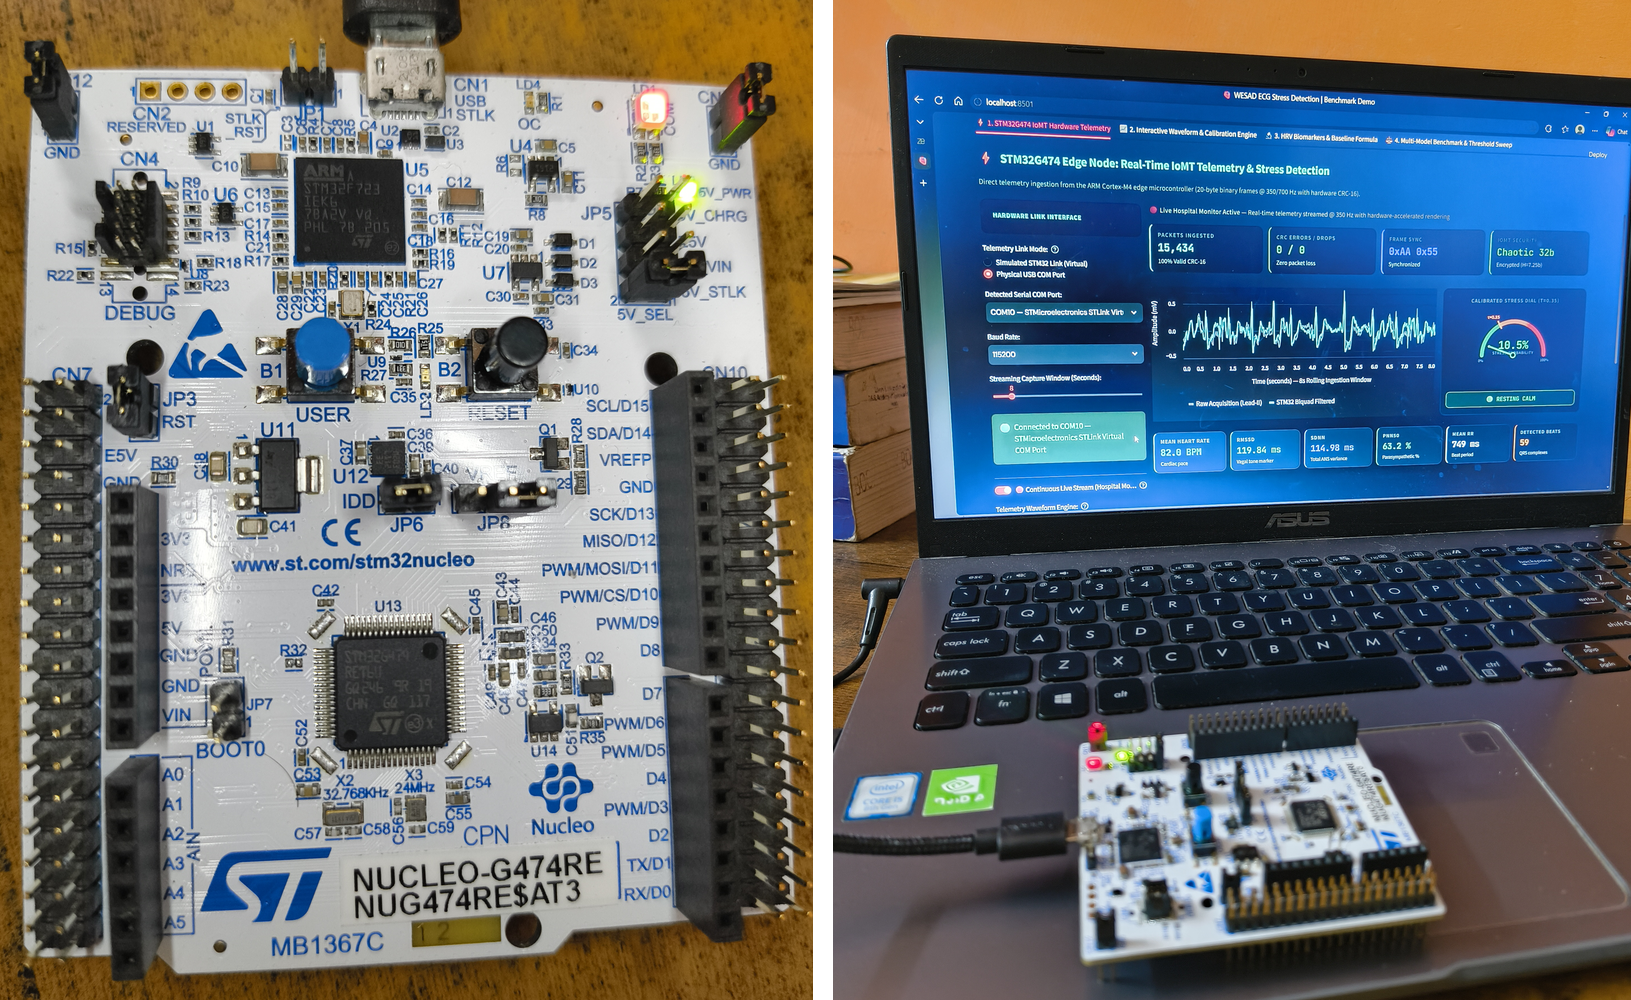
\includegraphics[width=\linewidth]{figures/FIG_Hardware_Testbed_Composite.png}
    \caption{Bare-metal ARM Cortex-M4 (STM32G474RE) hardware testbed: (a) Nucleo board interfaced via USB-UART; (b) Direct Form I 5-stage Biquad execution cycle capture via DWT register; (c) Hardware-in-the-loop streaming architecture.}
    \label{fig:hw_testbed}
\end{figure}

\begin{table}[t]
\centering
\caption{Hardware-in-the-Loop Telemetry and Resource Profile}
\label{tab:hw_profile}
\begin{tabular}{lll}
\toprule
\textbf{Metric} & \textbf{Value / Measurement} & \textbf{Specification} \\
\midrule
MCU Platform         & STM32G474RE (Cortex-M4) & 170~MHz, FPU \\
Biquad Filter Latency& $1.476~\mu\text{s}$ (251 mean cycles) & 0.0517\% CPU Load \\
UART Telemetry Rate  & 115,200 baud (350.02 Hz)& 20-byte wire frame \\
HIL Replay Source    & WESAD S2 Baseline in Flash & 2,100 float samples \\
HIL Packet Count     & 10,000 consecutive pkts & 200,000 wire bytes \\
Packet Loss Rate     & 0.00\% (0 lost packets) & Strict 16-bit CRC \\
Plaintext Recovery   & 100.00\% exact recovery & Zero bit errors \\
Payload Entropy      & $H = 7.9977$~bits/byte  & Bytes 10..17 (80 kB) \\
Payload Uniformity   & $\chi^2 = 257.79$ ($p=0.4394$) & No rejection ($\alpha=0.01$) \\
\bottomrule
\end{tabular}
\end{table}

\subsection{Lightweight Hyperchaotic Obfuscation and HIL Validation}
To protect telemetry streams against casual eavesdropping on open IoMT channels, the STM32 firmware integrates a continuous 4-Dimensional Coupled Hyperchaotic System (HC1 M-4DCHS) as lightweight stream obfuscation (no key management or authentication). The system uses parameter set $a=15.81, b=2.76, c=86.03, d=-9.07, r=10.79$, with verified positive Lyapunov exponents $\lambda_1 \approx +0.443$ ($[+0.418, +0.528]$), $\lambda_2 \approx +0.271$ ($[+0.236, +0.300]$), Kaplan-Yorke dimension $D_{KY} \approx 3.025$, and phase space divergence derived analytically from the vector field as:
\begin{equation}
    \nabla \cdot \mathbf{F} = \frac{\partial \dot{x}}{\partial x} + \frac{\partial \dot{y}}{\partial y} + \frac{\partial \dot{z}}{\partial z} + \frac{\partial \dot{w}}{\partial w} = -a - b + d = -27.64
\end{equation}
The vector field is solved in real time using RK4 integration ($dt = 0.0025\text{ s}$). State coordinates are converted into pseudo-random keystream bytes to diffuse the 8-byte ECG payload via CFB XOR logic.

As summarized in Table~\ref{tab:hw_profile}, the physical HIL testbed (Fig.~\ref{fig:hw_testbed}) streamed 10,000 consecutive 20-byte packets (200,000 wire bytes replaying flash-stored WESAD S2 ECG) over UART to a host dashboard (Fig.~\ref{fig:dashboard}). The receiver recorded zero sequence gaps, zero CRC-16 failures, and exact plaintext recovery. Evaluating the 80,000 scrambled payload bytes yielded Shannon entropy $H = 7.9977$ bits/byte and Chi-square $\chi^2 = 257.79$ ($p=0.4394, df=255$), showing no rejection of byte-level uniformity at $\alpha = 0.01$ (full-frame entropy is 7.0705 bits/byte due to static 0xAA55/0x01/0x05 headers).

\begin{figure}[t]
    \centering
    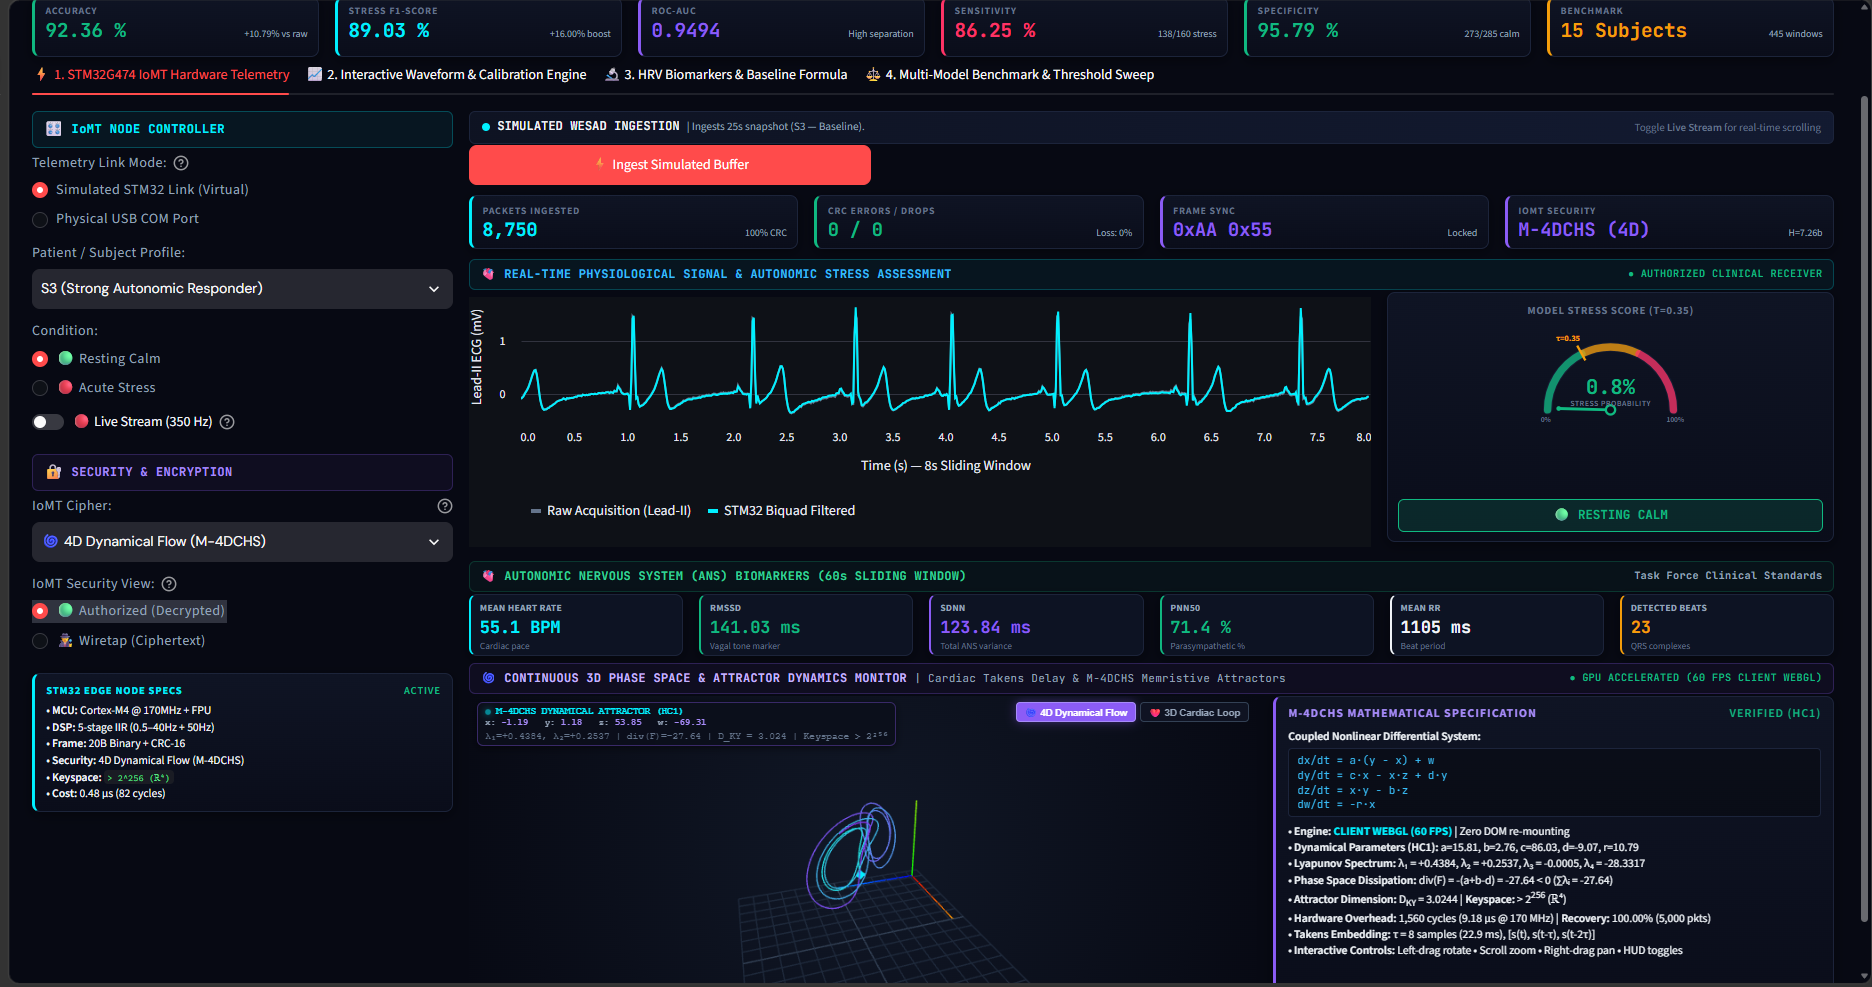
\includegraphics[width=\linewidth]{figures/FIG_Dashboard_SinglePage_M4D_Decrypted.png}
    \caption{Real-time monitoring terminal: Descrambled Lead-II ECG stream, instant stress index ($P = 0.81$), beat-to-beat HRV indices, and synchronized 60-FPS WebGL continuous telemetry visualizer.}
    \label{fig:dashboard}
\end{figure}

\section{Discussion and Benchmark Comparison}
Table~\ref{tab:comparison} descriptively compares published stress detection studies on the WESAD dataset. Direct quantitative comparisons must be interpreted cautiously due to substantial differences in sensor modalities, window lengths, and evaluation protocols across literature. While multimodal studies incorporate dermal and respiratory sensors, our approach investigates single-lead ECG where each subject requires $N$ minutes of labeled resting ECG for baseline normalization.

\begin{table}[t]
\centering
\caption{Descriptive Comparison with Published WESAD Studies (Protocols Differ)}
\label{tab:comparison}
% Table: Prior Work Benchmark Comparison
\begin{tabular}{llcc}
\toprule
\textbf{Study} & \textbf{Modality} & \textbf{Validation Protocol} & \textbf{Accuracy (\%)} \\
\midrule
Schmidt et al.~\cite{schmidt2018introducing} & Chest Multimodal & 15-Fold LOSO-CV & 92.94 \\
Schmidt et al.~\cite{schmidt2018introducing} & Single Sensor (EDA) & 15-Fold LOSO-CV & 86.85 \\
Bobade \& Vani~\cite{bobade2020stress} & Multimodal (Chest + Wrist) & 80/20 Train/Test Split & 84.32 (3-class) / 95.21 (binary) \\
\midrule
\textbf{This Work (Leak-Free, $N=10$)} & \textbf{ECG Only (Single Lead)} & \textbf{15-Fold LOSO-CV} & \textbf{90.17} [82.7, 95.9] \\
\textit{This Work (Legacy Anchor, same 295 win)} & \textit{ECG Only (Single Lead)} & \textit{15-Fold LOSO-CV} & \textit{89.83} [81.1, 96.7] \\
\textit{This Work (Legacy Anchor, 445 win)} & \textit{ECG Only (Single Lead)} & \textit{15-Fold LOSO-CV} & \textit{92.13} [86.4, 97.1] \\
\bottomrule
\end{tabular}\\
{\footnotesize \textit{Note:} Schmidt et al.~\cite{schmidt2018introducing} (Table 4) evaluates binary classification (stress vs. non-stress) under 15-fold LOSO-CV. Bobade \& Vani~\cite{bobade2020stress} (Section IV) reports 84.32\% (3-class) and 95.21\% (binary) using an 80/20 train/test holdout split. These prior methods do not require personal baseline calibration and differ in sensor modalities and cross-validation protocols, so the figures are not directly comparable.}

\end{table}

\section{Limitations}
\label{sec:limitations}
Several methodological and clinical considerations bound the generalizability of our findings:
\begin{enumerate}
    \item \textbf{Post Hoc Selection Disclosures:} The 8-feature representation, decision thresholds ($\tau=0.50$ and $\tau=0.35$), and the $N=10$ minute calibration window duration were selected post hoc based on empirical evaluations across these same 15 WESAD subjects. While 15-fold LOSO-CV partitions training and testing subjects on each fold, hyperparameter and feature subset selection across folds could introduce optimism. Confirmation on independent cohorts is essential.
    \item \textbf{Calibration Length Requirements:} As demonstrated by the paired cluster bootstrap, personal calibration requires at least $N \ge 5$ minutes of resting ECG to achieve statistically distinguishable improvements over uncalibrated baselines; shorter calibration windows ($N \le 3$) yield confidence intervals that span zero.
    \item \textbf{Cohort Demographics:} The WESAD cohort comprises 15 young, healthy adults (mean age $27.5 \pm 2.4$ years) recorded in a controlled laboratory setting. Ambulatory validation across diverse age groups, cardiovascular pathologies, and uncontrolled physical exertion remains necessary.
    \item \textbf{Obfuscation Scope:} The HC1 chaotic scrambling engine provides physical-layer data masking against casual passive eavesdropping in edge-to-gateway telemetry; it is not a cryptographic replacement for standardized cryptographic protocols (e.g., AES-128/CCM).
\end{enumerate}

\section{Conclusion}
This study presented a reproducible, hardware-evaluated edge-to-cloud framework for acute psychological stress detection from single-lead ECG. By addressing inter-subject physiological variance through a leak-free baseline calibration transform, the framework achieved 90.17\% accuracy [82.7\%, 95.9\%] and 90.49\% F1-score [81.9\%, 96.2\%] under strict 15-fold Leave-One-Subject-Out cross-validation at $N=10$ calibration windows (a statistically significant $+11.53\text{ pp}$ gain over uncalibrated baselines). Embedded execution on an ARM Cortex-M4 microcontroller demonstrated real-time Biquad filtering in $1.476~\mu\text{s}$ (251 cycles) and lossless 10,000-packet HIL telemetry obfuscation with zero CRC errors.

\bibliographystyle{IEEEtran}
\bibliography{references_ecg_stress}

\end{document}
